\documentclass{article}
\usepackage[utf8]{inputenc}
\usepackage{graphicx}
\usepackage{amsmath }
\usepackage{amssymb}
\usepackage{subcaption}
\usepackage{float}
\usepackage{multirow}
\setcounter{section}{1}


\usepackage{cleveref} %referencing figures, equations and tables
\crefformat{figure}{Figure.~#2#1#3}
\crefformat{equation}{Eq.~#2#1#3}
\crefformat{table}{Table.~#2#1#3}
\crefformat{appendix}{Appendix.~#2#1#3}
\crefformat{section}{Section.~#2#1#3}

\title{Analytical and Experimental Comparison of Composite Laminate Elastic Properties}
\author{Amir Baharvand }
\date{}

\begin{document}

\maketitle

\tableofcontents

\section{Introduction}
Elastic properties play a critical role in defining the stress-strain relation or the so-called constitutive law. Accuracy in determining the elastic properties helps researchers predict the material behavior under different loading conditions. This report aims to provide a comparison between the elastic properties determined from the classical laminate theory and tensile testing. The test coupons are manufactured using the autoclave and vacuum infusion. The rule of mixture and the 10\%-rule are further invoked to compare with the CLT and experiment. Eventually, the first-ply failure is utilized to predict the factor of safety of the composite laminates. \\

This report is divided into the following sections. \cref{sect:burnoff} discusses the determination of fiber volume fraction. \cref{sec:elastic_properties} summarizes the calculation of the elastic properties from different methods. A discussion on the result and the difference in laminate quality using the autoclave and vacuum infusion are given in \cref{sec:discussion}. Finally, \cref{sec:failure} reviews calculation of the factor of safety.

\section{Burn off Analysis}\label{sect:burnoff}
\cref{tab:fiber_prop} and \cref{tab:resin_prop} list the mechanical properties of the fiber (AS-4 Carbon) and resin (Epoxy 3501-6) used in this study. The laminate stacking sequence is [$\pm45/0/90/0$]$_\text{s}$.

\begin{table}[H]
    \centering
    \begin{tabular}{lccc} \hline
        Property & Symbol & Unit & Value \\ \hline
        Density & $\rho_f$ & kg/cm$^3$ & 1.81 \\
        Longitudinal modulus & $E_{1f}$ & GPa & 235 \\
        Transverse modulus & $E_{2f}$ & GPa & 15 \\
        Shear modulus & $G_{12f}$ & GPa & 27 \\
        Poisson's ratio & $\nu_{12f}$ & - & 0.20 \\ \hline
    \end{tabular}
    \caption{AS-4 Carbon mechanical properties}
    \label{tab:fiber_prop}
\end{table}

\begin{table}[H]
    \centering
    \begin{tabular}{lccc} \hline
        Property & Symbol & Unit & Value \\ \hline
        Density & $\rho_m$ & kg/cm$^3$ & 1.27 \\
        Young's modulus & $E_m$ & GPa & 4.3 \\
        Shear modulus & $G_m$ & GPa & 1.6 \\
        Poisson's ratio & $\nu_{m}$ & - & 0.35 \\ \hline
    \end{tabular}
    \caption{Epoxy 3501-6 mechanical properties}
    \label{tab:resin_prop}
\end{table}

The burn off test was conducted according to ASTM D3171-22 \cite{ASTMD3171}, method 1 procedure G. The crucible mass is 15 g and the void content is assumed to be zero. The autoclave and vacuum infusion laminate density are 1.60g/cm$^3$ and 1.45g/cm$^3$, respectively. First, the mass of the dry fiber, $m_f$, (after burn off) is calculated by deducting the crucible mass from the mass post-burn off. Then, fiber weight fraction, $W_f$, and fiber volume fraction, $V_f$ are calculated according to \cref{eq:W_f} and \cref{eq:V_f}.

\begin{equation}
    W_m = \dfrac{m_f}{m_i} \times 100
    \label{eq:W_f}
\end{equation}

\begin{equation}
    V_f = \dfrac{m_f}{m_i} \dfrac{\rho_i}{\rho_f} \times 100
    \label{eq:V_f}
\end{equation}

where $m_i$ and $\rho_i$ are the composite mass (before burn off) and density and $\rho_f$ is the fiber density. Next, the resin weight fraction, $W_m$, and volume fraction, $V_m$ are calculated from \cref{eq:W_m} and \cref{eq:V_m}.

\begin{equation}
    W_m = \dfrac{m_i - m_f}{m_i} \times 100
    \label{eq:W_m}
\end{equation}

\begin{equation}
    V_m = 100 - V_f
    \label{eq:V_m}
\end{equation}

where $\rho_m$ is the resin density.

\cref{tab:ac_vf} and \cref{tab:vi_vf} summarize the fiber/resin volume fraction along with their mean and standard deviation (STD). The mean values of the fiber volume fraction are used in \cref{sec:elastic_properties} to calculate the elastic properties. The small value of STD indicates the high precision of the burn off test. Further discussion on the accuracy of the test result is given in \cref{sec:elastic_properties}.

\begin{table}[h]
\centering
\caption{The autoclave laminate fiber/resin volume fraction.}
\label{tab:ac_vf}
\resizebox{\textwidth}{!}{\begin{tabular}{ccccccccc}
\hline
\multicolumn{1}{l}{Specimen} & \begin{tabular}[c]{@{}c@{}}Post-Burnoff mass \\ (crucible+contents) {[}g{]}\end{tabular} & \begin{tabular}[c]{@{}c@{}}Crucible \\ mass {[}g{]}\end{tabular} & \begin{tabular}[c]{@{}c@{}}$m_f$\\ {[}m{]}\end{tabular} & \begin{tabular}[c]{@{}c@{}}$m_c$\\ {[}m{]}\end{tabular} & $W_f$ [\%]   & $V_f$ [\%]   & $W_m$ [\%]   & $V_m$ [\%]   \\ \hline
1                            & 80.0                                                                                     & 15.0                                                             & 65.0                                                    & 94.0                                                    & 69.1489 & 61.1261 & 30.8511 & 38.8739 \\
2                            & 74.0                                                                                     & 15.0                                                             & 59.0                                                    & 85.3                                                    & 69.4118 & 61.3585 & 30.5882 & 38.6415 \\
3                            & 76.0                                                                                     & 15.0                                                             & 61.0                                                    & 88.2                                                    & 69.3182 & 61.2757 & 30.6818 & 38.7243 \\ \cline{6-9} 
                             &                                                                                          &                                                                  &                                                         &                                                         & Mean    & 61.25   &         & 38.75   \\
                             &                                                                                          &                                                                  &                                                         &                                                         & STD     & 0.12    &         & 0.12    \\ \hline
\end{tabular}}
\end{table}

\begin{table}[h]
\centering
\caption{The vacuum infusion laminate fiber/resin volume fraction.}
\label{tab:vi_vf}
\resizebox{\textwidth}{!}{\begin{tabular}{ccccccccc}
\hline
\multicolumn{1}{l}{Specimen} & \begin{tabular}[c]{@{}c@{}}Post-Burnoff mass \\ (crucible+contents) {[}g{]}\end{tabular} & \begin{tabular}[c]{@{}c@{}}Crucible \\ mass {[}g{]}\end{tabular} & \begin{tabular}[c]{@{}c@{}}$m_f$\\ {[}m{]}\end{tabular} & \begin{tabular}[c]{@{}c@{}}$m_c$\\ {[}m{]}\end{tabular} & $W_f$ [\%]   & $V_f$ [\%]   & $W_m$ [\%]   & $V_m$ [\%]   \\ \hline
1                            & 89.0                                                                                     & 15.0                                                             & 74.0                                                    & 172.0                                                   & 43.0233 & 34.4661 & 56.9767 & 65.5339 \\
2                            & 84.0                                                                                     & 15.0                                                             & 69.0                                                    & 166.0                                                   & 41.5663 & 33.2989 & 58.4337 & 66.7011 \\
3                            & 78.0                                                                                     & 15.0                                                             & 63.0                                                    & 154.0                                                   & 40.9091 & 32.7725 & 59.0909 & 67.2275 \\ \cline{6-9} 
                             &                                                                                          &                                                                  &                                                         &                                                         & Mean    & 33.51   &         & 66.49   \\
                             &                                                                                          &                                                                  &                                                         &                                                         & STD     & 0.87    &         & 0.87    \\ \hline
\end{tabular}}
\end{table}

\section{Elastic Properties} \label{sec:elastic_properties}
\subsection{Rule of Mixture}
The rule of mixture (ROM) assumes unidirectional fibers for the determination of lamina properties; however, in case of a laminate with different fiber angles, the ROM is incapable of yielding correct values. This is due to the lack of contribution of each ply to a certain property. For instance, the contribution from $\pm\theta$ and 90$^o$ is not the same as 0$^o$ plies in axial loading. The contribution of each ply can be determined using the so-called Krenchel orientation efficiency factor, $\eta_{\theta}$ \cite{krenchel1964fibre} and is defined according to \cref{eq:krenchel}.

\begin{equation}
    \eta_{\theta} = \displaystyle\sum a_n \cos^4(\theta_n)
    \label{eq:krenchel}
\end{equation}

where $a_n$ is the fraction of layers with orientation angle $\theta_n$ with respect to the loading direction. Rewriting the ROM using Krenchel orientation efficiency factor gives

\begin{flalign}
    & E_x = \eta_{\theta 1} E_f V_f + E_m (1 - V_f) \notag \\
    & E_y = \eta_{\theta 2} E_f V_f + E_m (1 - V_f) 
    \label{eq:rom_krenchel}
\end{flalign}

in which $E_x$ and $E_y$ are the laminate longitudinal and transverse elastic modulus. $\eta_{\theta}$ values are tabulated in \cref{tab:eta_rom}. It can be seen that the contribution of $90^o$ to the longitudinal elastic modulus is zero. Similarly, $0^o$ plies have no effect on the transverse elastic modulus.

\begin{table}[h]
\centering
\begin{tabular}{lccclccclll}
\cline{2-11}
              & \multicolumn{3}{c}{$a_n$}  &  & \multicolumn{3}{c}{$\cos^4(\theta)$} &  & \multirow{2}{*}{$\eta_{\theta1}$} & \multirow{2}{*}{$\eta_{\theta2}$} \\ \cline{2-4} \cline{6-8}
              & $0^o$ & $90^o$ & $\pm45^o$ &  & $0^o$     & $90^o$    & $\pm45^o$    &  &                                   &                                   \\ \hline
$x$-direction & 0.4   & 0.2    & 0.4       &  & 1         & 0         & 0.25         &  & \multicolumn{1}{c}{0.5}           & \multicolumn{1}{c}{-}             \\
$y$-direction & 0.4   & 0.2    & 0.4       &  & 0         & 1         & 0.25         &  & \multicolumn{1}{c}{-}             & \multicolumn{1}{c}{0.3}           \\ \hline
\end{tabular}
\caption{$\eta_{\theta}$ values for determination of the longitudinal and transverse elastic modulus using the ROM.}
\label{tab:eta_rom}
\end{table}

\subsection{10\%-Rule}
The 10\%-rule \cite{HartSmith1992} provides a quick and reliable initial estimation of elastic properties in composite laminates and is popular in the aerospace industry where most of the laminate include $0^o$, $90^o$ and $\pm45^o$. According to this rule, the contribution of the $\pm45^o$ and $90^o$ plies to the overall laminate elastic modulus is one-tenth of a $0^o$ ply in axial loading. Similarly, $0^o$ and $90^o$ plies contribute one-tenth of an equivalent $\pm45^o$ ply to the in-plane shear modulus. Therefore, the 10\%-rule can be summarized as 

\begin{flalign}
    & E_x = E_{11} (0.1 + 0.9 \lambda_0) \notag \\
    & E_y = E_{11} (0.1 + 0.9 \lambda_{90}) \notag \\
    & \mu_{xy} = G_{12} (0.025 + 0.234 \lambda_{\pm45})
    \label{eq:ten_percent}
\end{flalign}

where

\begin{flalign}
    & E_{11} = E_f V_f + E_m (1 - V_f) \notag \\
    & \dfrac{1}{G_{12}} = \dfrac{V_f}{G_f} + \dfrac{(1 - V_f)}{G_m} \notag
    % \label{}
\end{flalign}

$E_{11}$ is the longitudinal modulus, $G_{12}$ and $\mu_{xy}$ are the fiber and laminate in-plane shear modulus, $\lambda_0$, $\lambda_{90}$ and $\lambda_{\pm45}$ denote the fraction of $0^o$, $90^o$ and $\pm45^o$ plies. For the given stacking sequence, $\lambda_0 = 0.4$, $\lambda_{90} = 0.2$ and $\lambda_{\pm45} = 0.4$.

\subsection{Classical Laminate Theory (CLT)}
\cref{fig:clt_algorithm} summarizes the approach utilized by the CLT. The left column is known as the $ABD$ matrix, which connects the applied force/moment to strain/curvature. The right column solves for the global strain/curvature of the laminate using the $ABD$ matrix and the applied force/moment. Global stress is determined using the constitutive law (stress-strain relation) and the strain and stress of each ply are calculated using the transformation of their corresponding global values.

\begin{figure}[h]
    \centering
    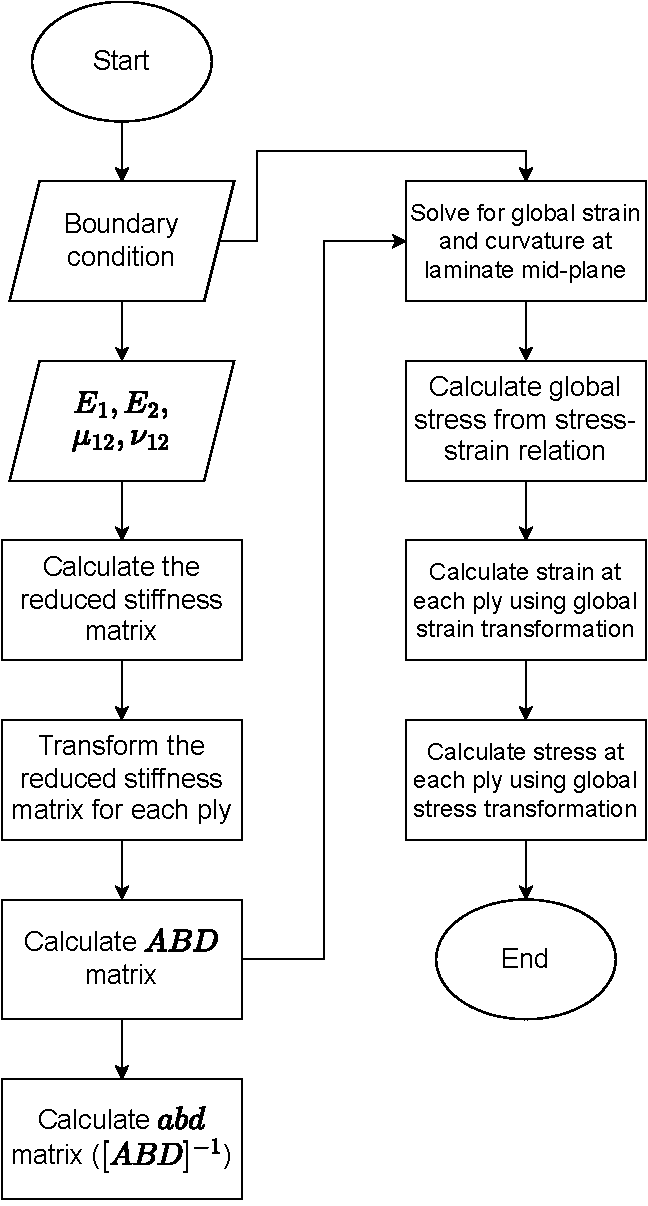
\includegraphics[width=0.5\textwidth]{figures/clt_algorithm.pdf}
    \caption{The composite laminate theory (CLT) flowchart.}
    \label{fig:clt_algorithm}
\end{figure}

\section{Discussion}\label{sec:discussion}
As expected, the result from \cref{sect:burnoff} shows a higher fiber volume fraction for the autoclave laminate. The process from vacuum bagging to curing in an autoclave is performed inside a pressurized vessel under controlled temperature and pressure. The pressurized vessel increases the compaction between the vacuum bag and fibers, leading to minimum void and high fiber content. In contrast, the vacuum infusion uses atmospheric pressure for compaction, leading to a higher void content and lower fiber volume fraction in comparison to the autoclave. Furthermore, in vacuum infusion, the curing is usually performed at room temperature or after infusion, in an oven which complicates the curing parameters. As a result, the mechanical properties of a laminate manufactured using the vacuum infusion are inferior to the autoclave. \\

\cref{tab:elastic_prop_ac} and \cref{tab:elastic_prop_vi} list the elastic properties of the autoclave and vacuum infusion laminates using different methods. A noticeable difference in the longitudinal elastic modulus of the autoclave laminate between the analytical and experimental results is visible. Despite the high volume fraction of the autoclave laminate (61.25\%), there is a noticeable difference of 18.4\% between the measured $E_{x}$ and the CLT result. Several reasons might have caused this discrepancy. The misalignment in the tensile testing machine results in an underestimated value of $E_{x}$. Another reason could be the presence of delamination in the testing coupon due to improper manufacturing. Hence, inspection using the non-destructive testing method, \emph{i.e.}, C-scan of the manufactured laminates for detecting defects like delamination, is recommended \cite{Imielinska2004}. Furthermore, he fiber and resin volume fraction from \cref{tab:ac_vf} shows high fiber content in the autoclave laminate which contradicts the experimental results of $E_x$. This contradiction concludes the presence of local delamination in the autoclave laminate, being more pronounced in the region where the tensile testing coupons are cut. While the ROM and CLT can predict the transverse elastic modulus, $E_y$, the 10\%-rule gives a lower value. The difference between the analytical and experimental values for the shear modulus and Poisson's ratio is negligible, which shows the advantage of the 10\%-rule in predicting the shear modulus and Poisson's ratio of the multi-axial laminate with less computational effort than the CLT. \\

\begin{table}[h]
\resizebox{\textwidth}{!}{\begin{tabular}{lccccccc}
\hline
Elastic properties           & Symbol     & Unit & ROM    & 10\%-rule & CLT & Experiment & COV [\%]\\ \hline
& & & & & & \\
Longitudinal elastic modulus & $E_{x}$    & GPa & 73.635(20.3) & 66.978(9.4) & 72.436(18.4) & $61.2^{61.9}_{60.5}$ & 1.2\\
& & & & & & & \\
Transverse elastic modulus   & $E_{y}$    & GPa & 44.848(-1.4) & 40.769(-10.4) & 46.473(2.1) & $45.5^{47.5}_{43.5}$ & 4.3\\
& & & & & & & \\
In-plane shear modulus       & $\mu_{xy}$   & GPa & - & 17.293(0) & 17.238(0) & $16.8^{17.8}_{15.8}$ & 6.1\\
& & & & & & & \\
In-plane Poisson's ratio     & $\nu_{xy}$ & -    & - & - & 0.3118(0) & $0.31^{0.32}_{0.30}$ & 2.4\\ 
& & & & & & & \\ \hline
\end{tabular}}
\caption{Comparison of the autoclave laminate elastic properties using different methods (numbers in parentheses indicate the relative difference with the experiment)}
\label{tab:elastic_prop_ac}
\end{table}

The analytical results from the vacuum infusion show a good agreement with the experiment. The maximum difference is 13.8\% for the transverse elastic modulus using the 10\%-rule. This implies a uniform distribution of fibers through the laminate and good manufacturing quality. 

\begin{table}[h]
\resizebox{\textwidth}{!}{\begin{tabular}{lccccccc}
\hline
Elastic properties           & Symbol     & Unit & ROM    & 10\%-rule & CLT & Experiment & COV [\%]\\ \hline
& & & & & & & \\
Longitudinal elastic modulus & $E_{x}$ & GPa & 48.165(5.6) & 37.539(-6.2) & 41.084(2.7) & $40^{41.8}_{38.2}$ & 4.5\\
& & & & & & & \\
Transverse elastic modulus   & $E_{y}$ & GPa & 29.953(-0.1) & 22.850(-13.8) & 26.822(1.2) & $26.5^{28.5}_{24.5}$ & 7.4\\
& & & & & & & \\
In-plane shear modulus       & $\mu_{xy}$ & GPa & - & 10.700(0) & 9.835(0) & $9.82^{10.63}_{9.01}$ & 8.2\\
& & & & & & & \\
In-plane Poisson's ratio     & $\nu_{xy}$ & -    & - & - & 0.3205(0) & $0.31^{0.32}_{0.30}$ & 3.1\\
& & & & & & & \\ \hline
\end{tabular}}
\caption{Comparison of the infused laminate elastic properties using different methods (numbers in parentheses indicate the relative difference with the experiment).}
\label{tab:elastic_prop_vi}
\end{table}

The predicted and measured elastic properties are plotted in \cref{fig:elastic_properties_envelope}. The result shows the conservative nature of the 10\%-rule in comparison to the ROM and CLT and the application of the 10\%-rule for a quick estimation of the elastic properties of the multi-axial laminates.

\begin{figure}[h]
    \begin{subfigure}{0.5\textwidth}
        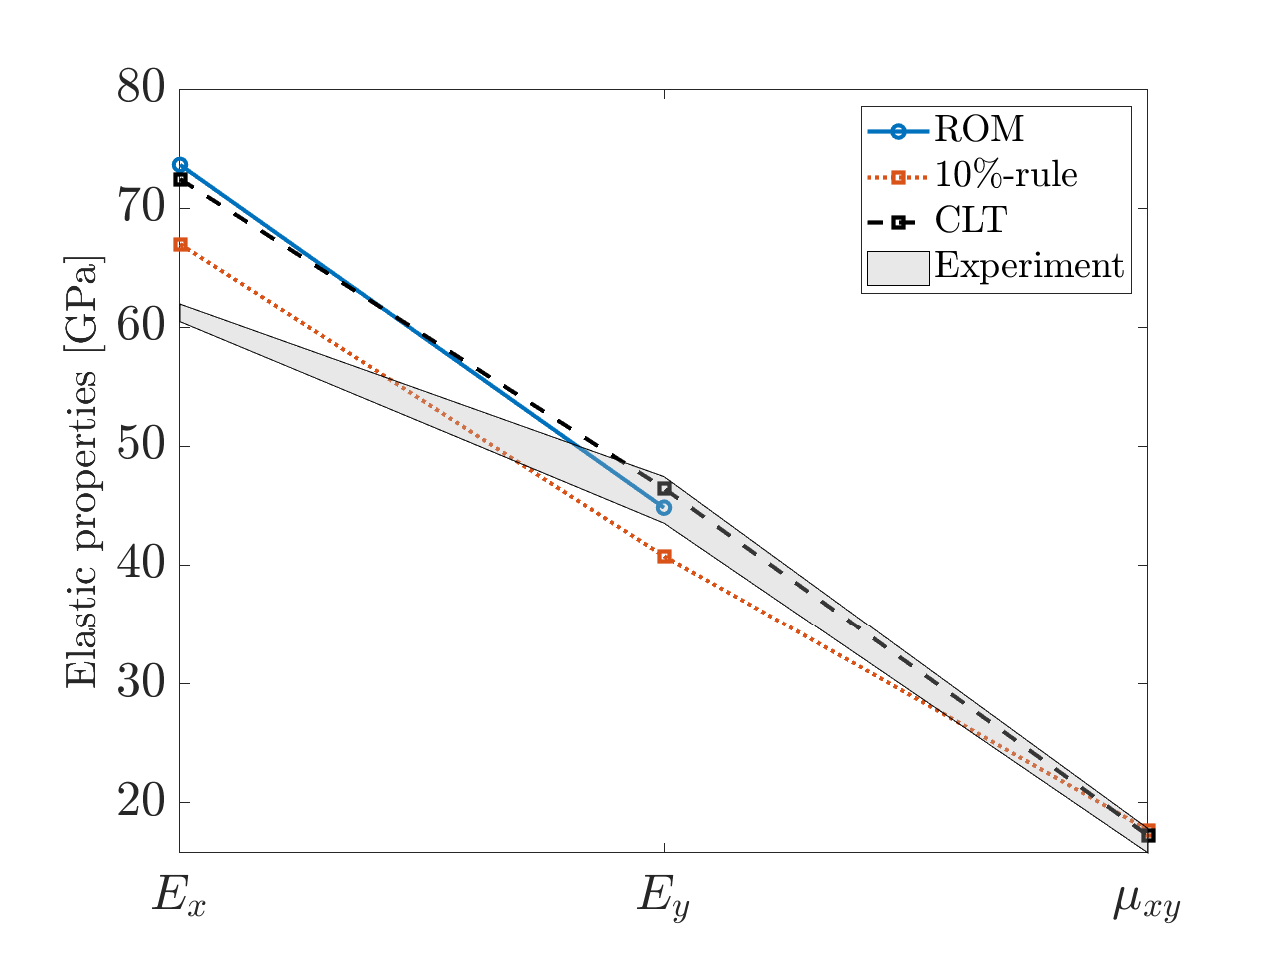
\includegraphics[width=1\linewidth, height=0.8\linewidth]{figures/autoclave.eps} 
        \caption{Autoclave.}
        % \label{fig:autoclave}
    \end{subfigure}
    \begin{subfigure}{0.5\textwidth}
        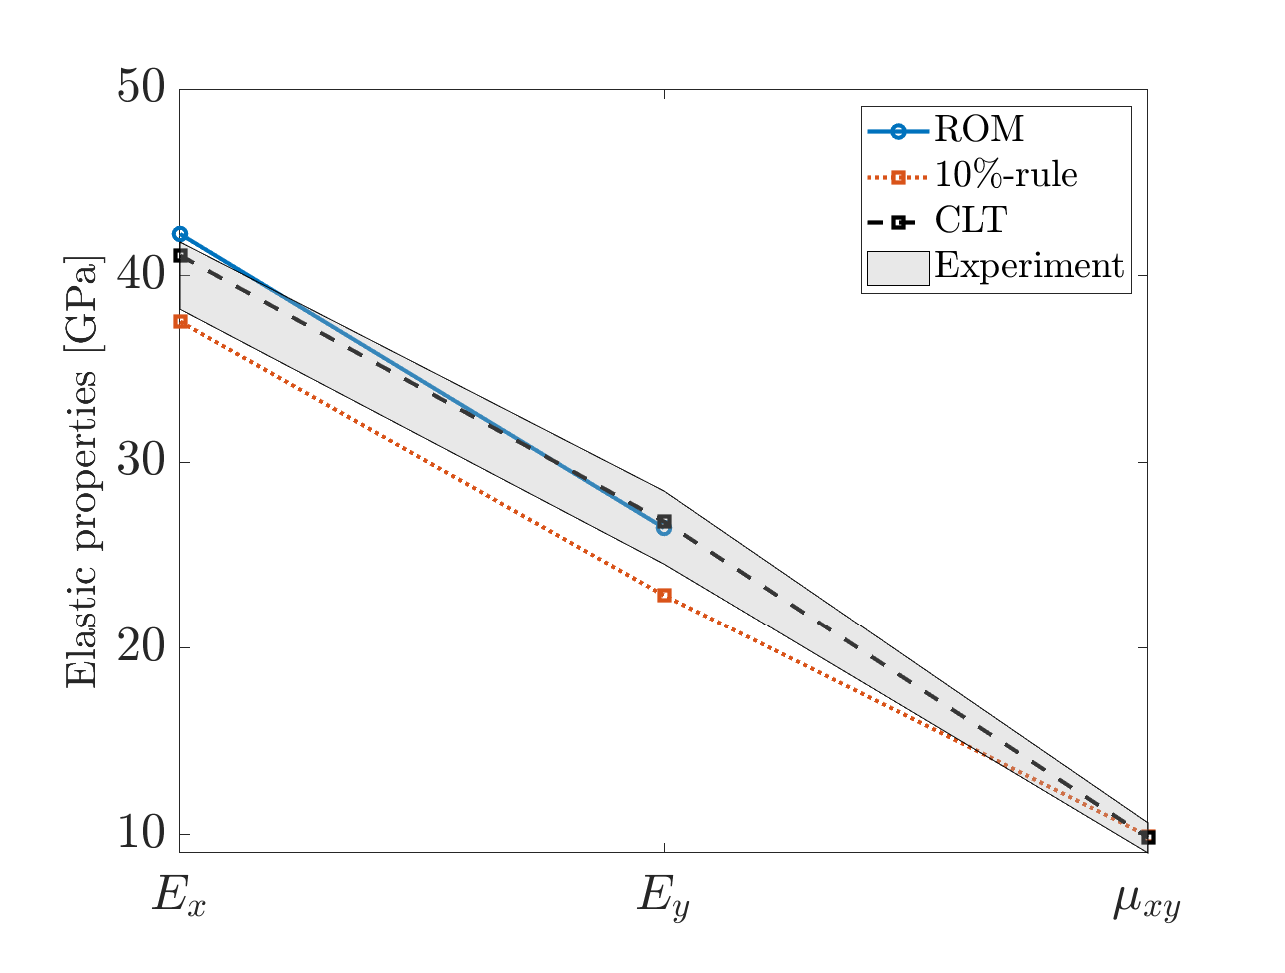
\includegraphics[width=1\linewidth, height=0.8\linewidth]{figures/vacuum_infusion.eps} 
        \caption{Vacuum infusion.}
        % \label{fig:vacuum_infusion}
    \end{subfigure}
    \caption{Analytical and experimental elastic properties comparison.}
    \label{fig:elastic_properties_envelope}
\end{figure}

\section{Laminate Factor of Safety}\label{sec:failure}
The methodology for determination of the factor of safety (S.F) in the present report is based on the failure index (F.I) in the first ply failure. \cref{tab:strength} lists the strength values of the autoclave and vacuum infusion laminates. It is worth noting that the worst-case scenario (lower bound of the strength values) is used for calculating the factor of safety for each laminate. The applied stress is integrated through the laminate thickness to convert them into stress resultant.

\begin{table}[H]
\resizebox{\textwidth}{!}{\begin{tabular}{lcccclcc} \hline
\multirow{2}{*}{Property}         & \multicolumn{1}{l}{\multirow{2}{*}{Symbol}} & \multicolumn{1}{l}{\multirow{2}{*}{Unit}} & \multicolumn{2}{c}{Autoclave} &  & \multicolumn{2}{c}{Vacuum infusion} \\ \cline{4-5} \cline{7-8} 
                                  & \multicolumn{1}{l}{}                        & \multicolumn{1}{l}{}                      & Value      & COV{[}\%{]}      &  & Value         & COV{[}\%{]}         \\ \hline
Longitudinal tensile strength     & $X_t$                                       & MPa                                       & 2200       & 1.2              &  & 2050          & 3.7                 \\
Longitudinal compressive strength & $Y_c$                                       & MPa                                       & 2350       & 16               &  & 2300          & 23                  \\
Transverse tensile strength       & $Y_t$                                       & MPa                                       & 50         & 2.8              &  & 42            & 6.1                 \\
Transverse tensile strength       & $Y_c$                                       & MPa                                       & 56         & 17               &  & 51            & 25                  \\
In-plane shear strength           & $S$                                         & MPa                                       & 72         & 7.6              &  & 68            & 12                  \\ \hline            
\end{tabular}}
    \caption{Strength values of the autoclave and vacuum infusion laminates in different directions.}
    \label{tab:strength}
\end{table}

\subsection{Maximum Strain and Maximum Stress}
According to the maximum strain theory, failure occurs when the strain at one ply exceeds the ultimate strain. The failure index for this theory is 

\begin{equation}
    \text{F.I} = \max\{\text{abs}\{\dfrac{\epsilon_{11}}{eX_t}, \dfrac{\epsilon_{11}}{eX_c}, \dfrac{\epsilon_{22}}{eY_t}, \dfrac{\epsilon_{22}}{eY_c}, \dfrac{\epsilon_{12}}{eS}\}\}
    \label{eq:max_strain_fi}
\end{equation}

where $eX$, $eY$ and $eS$ are the ultimate longitudinal, transverse and in-plane strain, subscripts $t$ and $c$ indicate the tension and compression, 1, 2 and 3 designate the ply coordinate system, $\epsilon$ is the strain and "max" and "abs" are the maximum and absolute. Similarly, for the maximum stress theory, failure happens when the stress in a ply reaches the ultimate strength; hence, the failure index for the maximum stress can be defined as 

\begin{equation}
    \text{F.I} = \max\{\text{abs}\{\dfrac{\sigma_{11}}{X_t}, \dfrac{\sigma_{11}}{X_c}, \dfrac{\sigma_{22}}{Y_t}, \dfrac{\sigma_{22}}{Y_c}, \dfrac{\sigma_{12}}{S}\}\}
    \label{eq:max_stress_fi}
\end{equation}

where $X$, $Y$ and $S$ are the ply ultimate longitudinal, transverse and in-plane strength and $\sigma$ is the local stress. Hence, the factor of safety for the maximum strain and maximum stress failure criteria is \cite{helius}

\begin{equation}
    \text{S.F} = \min\{\dfrac{1}{\text{F.I}}\}
    \label{eq:max_strain_stress_sf}
\end{equation}

Please see \cref{sec:eLamX} for a comment on the result drom maximum strain theory.

\subsection{Tsai-Hill}
According to Tsai-Hill failure criterion, failure occurs when 

\begin{equation}
    \text{F.I} = \dfrac{\sigma_{11}^2}{X^2} + \dfrac{\sigma_{22}^2}{Y^2} - \dfrac{\sigma_{11} \sigma_{22}}{X^2} + \dfrac{\sigma_{12}^2}{S^2} \geq 1
    \label{eq:tsai_hill_fi}
\end{equation}

where $X$ and $Y$ are the tensile/compressive strength and change signs accordingly, \emph{i.e.} in case of compressive stress, $X$ and $Y$ become $X_c$ and $Y_c$. Hence, the factor of safety becomes \cite{helius}

\begin{equation}
    \text{S.F} = \sqrt{\dfrac{1}{\dfrac{\sigma_{11}^2}{X^2} + \dfrac{\sigma_{22}^2}{Y^2} - \dfrac{\sigma_{11} \sigma_{22}}{X^2} + \dfrac{\sigma_{12}^2}{S^2}}}
    \label{eq:tsai_hill_sf}
\end{equation}

\subsection{Hashin}
The implemented Hashin excludes the coupling between the normal and in-plane shear stress \cite{Hashin2016}. Hashin failure criterion differentiates between the fiber and matrix failure; therefore, two failure indices are defined according to \cref{eq:hashin_fi}.

\begin{flalign}
    & \text{(F.I)$_{\text{f}}$} = \dfrac{\sigma_{11}^2}{X^2} \geq 1 \notag \\
    & \text{(F.I)$_{\text{m}}$} =  \dfrac{\sigma_{22}^2}{Y^2} + \dfrac{\sigma_{12}^2}{S^2} \geq 
    1
    \label{eq:hashin_fi}
\end{flalign}

where the former is for the fiber and the latter is for the matrix failure. Similar to Tsai-Hill, the factors of safety for the fiber and matrix become

\begin{flalign}
    & \text{(S.F)$_{\text{f}}$} = \sqrt{\dfrac{1}{\text{(F.I)$_{\text{f}}$}}} \notag \\
    & \text{(S.F)$_{\text{m}}$} =  \sqrt{\dfrac{1}{\text{(F.I)$_{\text{m}}$}}} \notag
    % \label{}
\end{flalign}

The final factor of safety is the minimum of (S.F)$_{\text{f}}$ and (S.F)$_{\text{m}}$.

\begin{equation}
    \text{S.F} = \min\{ \text{(S.F)$_{\text{f}}$}, \text{(S.F)$_{\text{m}}$} \}
\end{equation}

The factor of safety for five different load cases is presented in \cref{tab:sf_autoclave} and \cref{tab:sf_vacuum_infusion}. \cref{fig:failure_criteria_cmp_arrow} illustrates different failure criteria in this report. The maximum strain theory gives lower values of the factor of safety compared to the other. This difference is more pronounced in load case \#5. In this load case, both Hashin and maximum stress theories yield a similar result as the coupling between the shear and longitudinal stress, $\sigma_{11}$, is neglected in Hashin failure criterion \cite{Hashin2016}.

\begin{table}[H]
    \centering
    \resizebox{\textwidth}{!}{\begin{tabular}{clccccc} \hline
        Case \# & Description & \multicolumn{1}{c}{\begin{tabular}[c]{@{}c@{}}Magnitude\\ {[}MPa{]}\end{tabular}} & \multicolumn{1}{c}{\begin{tabular}[c]{@{}c@{}}Maximum\\ strain\end{tabular}} & \multicolumn{1}{c}{\begin{tabular}[c]{@{}c@{}}Maximum\\ stress\end{tabular}} & Tsai-Hill & Hashin \\ \hline
        1 & Longitudinal tension & 80 & 5.51 & 5.97 & 6.16 & 6.24 \\
        2 & Longitudinal compression & -65 & 6.78 & 7.35 & 7.28 & 7.35 \\
        3 & Transverse tension & 5 & 56.57 & 59.44 & 61.82 & 62.16 \\
        4 & Transverse compression & -5 & 56.57 & 59.44 & 59.20 & 59.44 \\
        5 & In-plane shear & 20 & 10.49 & 14.93 & 12.43 & 14.09 \\ \hline
    \end{tabular}}
    \caption{Factor of safety of each load case for the autoclave laminate.}
    \label{tab:sf_autoclave}
\end{table}

\begin{table}[H]
    \centering
    \resizebox{\textwidth}{!}{\begin{tabular}{clccccc} \hline
        Case \# & Description & \multicolumn{1}{c}{\begin{tabular}[c]{@{}c@{}}Magnitude\\ {[}MPa{]}\end{tabular}} & \multicolumn{1}{c}{\begin{tabular}[c]{@{}c@{}}Maximum\\ strain\end{tabular}} & \multicolumn{1}{c}{\begin{tabular}[c]{@{}c@{}}Maximum\\ stress\end{tabular}} & Tsai-Hill & Hashin \\ \hline
        1 & Longitudinal tension & 80 & 3.47 & 3.82 & 3.91 & 3.94\\
        2 & Longitudinal compression & -65 & 4.28 & 4.70 & 4.68 & 4.70 \\
        3 & Transverse tension & 5 & 36.31 & 38.50 & 39.59 & 39.70 \\
        4 & Transverse compression & -5 & 36.31 & 38.50 & 38.42 & 38.50 \\
        5 & In-plane shear & 20 & 6.66 & 9.44 & 8.77 & 9.45 \\ \hline
    \end{tabular}}
    \caption{Factor of safety of each load case for the vacuum infusion laminate.}
    \label{tab:sf_vacuum_infusion}
\end{table}

\begin{figure}[h]
    \centering
    \includegraphics[width=0.8\textwidth]{figures/failure_criteria_cmp_arrow.eps}
    \caption{An schematic representation of the failure criteria.}
    \label{fig:failure_criteria_cmp_arrow}
\end{figure}

\section{Conclusion}
A comparative study between analytical and experimental values of the elastic properties of two laminates manufactured using the autoclave and vacuum infusion is presented. The laminate manufactured using the autoclave shows superior mechanical properties compared to the vacuum infusion laminate. The autoclave's elastic properties and fiber volume fraction show almost a twofold increase, which justifies the application of this manufacturing method to the aerospace industry, where both strength and stiffness are important. The result shows a good agreement between the experiment and composite laminate theory. The 10\%-rule leads to a more conservative result compared to the rule of mixture and classical laminate theory. 


\newpage
\bibliography{ref}
\bibliographystyle{ieeetr}

\end{document}